\subsection{Filamentation}

The propagation of femtosecond laser pulses in transparent dielectrics such as $\mathrm{SiO}_2$ can lead to the formation of filaments. This self guided mecanism originate from a dynamic balance between Kerr self-focusing and plasma defocusing. This phenomenon occurs when the input power exceeds a critical value, denoted $P_{cr}$, is illustrated in Figure~\ref{fig:filamentation_schematic}.

\begin{figure}[h!]
    \centering
    \resizebox{\textwidth}{!}{%
    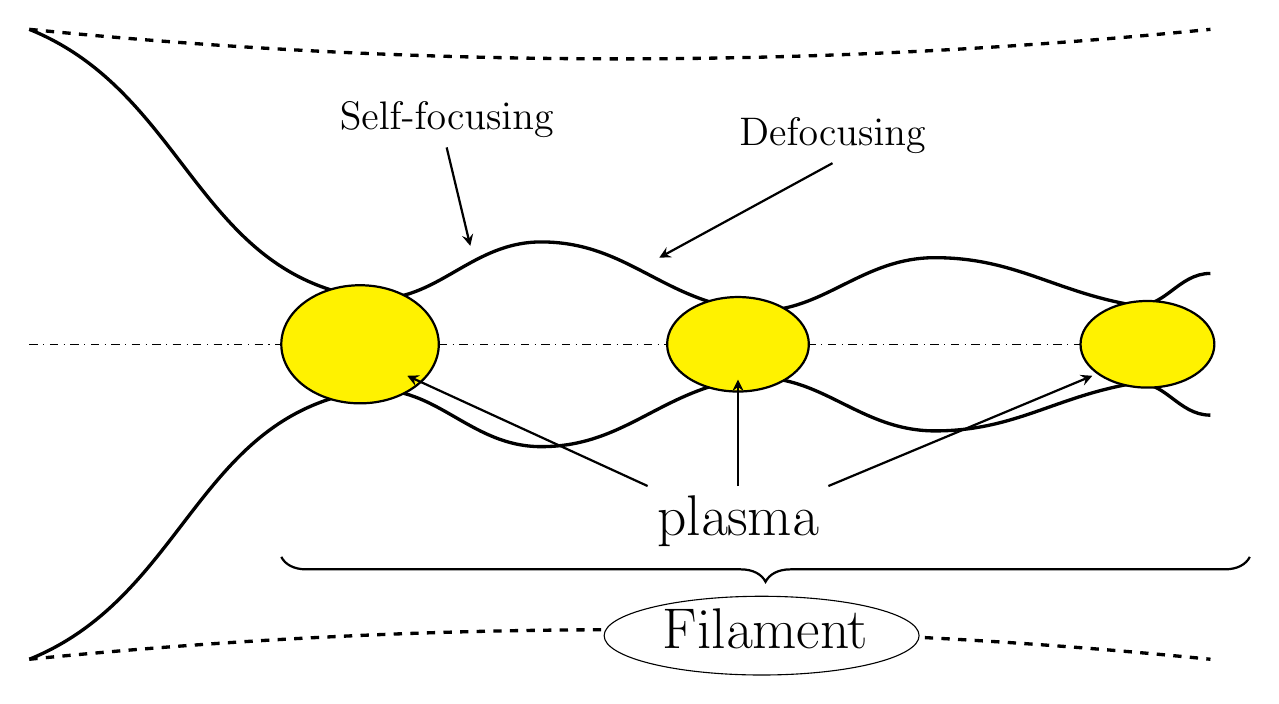
\begin{tikzpicture}[>=stealth]
        \def\xend{15}
        \def\ymax{4}

        \draw[dash dot, thin] (0,0) -- (\xend,0) [->];

        \draw[very thick, dashed] (0, \ymax) .. controls (5, 3.5) and (10, 3.5) .. (\xend, \ymax);
        \draw[very thick, dashed] (0, -\ymax) .. controls (5, -3.5) and (10, -3.5) .. (\xend, -\ymax);

        \draw[very thick] (0, \ymax)
            to[out=-22, in=170] (4.2, 0.6)
            to[out=-10, in=180] (6.5, 1.3)
            to[out=0, in=170]   (9.0, 0.45)
            to[out=-10, in=180] (11.5, 1.1)
            to[out=0, in=170]   (14.0, 0.5)
            to[out=-10, in=180] (\xend, 0.9);

        \draw[very thick] (0, -\ymax)
            to[out=22, in=-170] (4.2, -0.6)
            to[out=10, in=-180] (6.5, -1.3)
            to[out=0, in=-170]  (9.0, -0.45)
            to[out=10, in=-180] (11.5, -1.1)
            to[out=0, in=-170]  (14.0, -0.5)
            to[out=10, in=-180] (\xend, -0.9);
        \draw[fill=white] (9.3, -3.7 ) ellipse (2 and 0.50);
        \draw[fill=yellow, thick] (4.2, 0) ellipse (1.0 and 0.75);
        \draw[fill=yellow, thick] (9.0, 0) ellipse (0.9 and 0.6);
        \draw[fill=yellow, thick] (14.2, 0) ellipse (0.85 and 0.55);

        \node[above] (sf) at (5.3, 2.5) {\Large Self-focusing};
        \draw[->, thick] (sf.south) -- (5.6, 1.25);

        \node[above] (df) at (10.2, 2.3) {\Large Defocusing};
        \draw[->, thick] (df.south) -- (8.0, 1.1);

        \node[below] (plasma_text) at (9.0, -1.8) {\huge plasma};
        \draw[->, thick] (plasma_text.north west) -- (4.8, -0.4);
        \draw[->, thick] (plasma_text.north) -- (9.0, -0.45);
        \draw[->, thick] (plasma_text.north east) -- (13.5, -0.4);

        \draw[decorate, decoration={brace, amplitude=9pt, mirror}, thick]
            (3.2, -2.7) -- (15.5, -2.7) node[midway, below=15pt] {\huge Filament};
    \end{tikzpicture}%
    }
    \caption{Schematic beam envelope undergoing repeated cycles of Kerr self-focusing and plasma defocusing. Each collapse is arrested before catastrophic self-focusing by the free electron plasma generated near the intensity peak (yellow), which defocuses the beam until the intensity drops enough for the plasma to recombine and self-focusing to take over again, refilled by the surrounding energy reservoir. This repeated breathing over an extended propagation distance is the filament.}
    \label{fig:filamentation_schematic}
\end{figure}


The critical power $P_{cr}$ follows from the balance between the nonlinear self-focusing effect and diffraction. For a Gaussian beam, it is given by~\cite{marburger1975}:
\begin{equation}
    P_{cr} = \frac{3.77 \lambda_0^2}{8 \pi n_0 n_2},
\end{equation}
where $\lambda_0$ is the laser wavelength, $n_0$ the linear refractive index, and $n_2$ the nonlinear index coefficient. The numerical factor is $3.77$ for a Gaussian beam and $3.72$ for the Townes profile, for which diffraction and self-focusing balance exactly.

Above threshold, the distance at which an unopposed beam would collapse is given by the semi-empirical formula fitted to numerical solutions of the nonlinear Schr\"odinger equation by Dawes and Marburger~\cite{dawes1969,marburger1975}:
\begin{equation}
    \label{eq:marburger}
    L_c = \frac{0.367\, L_{DF}}{\sqrt{\big[(P_{in}/P_{cr})^{1/2} - 0.852\big]^2 - 0.0219}},
\end{equation}
where $L_{DF} = k_0 w_0^2 / 2$ is the Rayleigh length. For an externally focused beam of focal length $f$, the collapse distance shortens according to $L_{c,f}^{-1} = L_c^{-1} + f^{-1}$. Equation~\eqref{eq:marburger} is what sets the position of the nonlinear focus in the simulations, before plasma defocusing arrests the collapse.

For fused silica, typical values at $\lambda_0 = 800 \text{ nm}$ are $n_0 \approx 1.45$ and $n_2 \approx 2.4 \times 10^{-20} \text{ m}^2/\text{W}$, a value measured by Taylor et al. and reported in the reference compilation of Milam~\cite{milam1998}. Using these values, we calculate $P_{cr} \approx 2.8 \text{ MW}$, consistent with the $1.98$ to $2.5\text{ MW}$ reported respectively in~\cite{PhysRevB.71.125435} and~\cite{kandidov2009} for fused silica at this wavelength. At $\lambda_0 = 1030 \text{ nm}$, since no measurement exists exactly at this wavelength, we use the closest value available in the literature, $n_2 \approx 2.74 \times 10^{-20} \text{ m}^2/\text{W}$ at $1053\text{ nm}$~\cite{milam1998}, which gives $P_{cr} \approx 4.0 \text{ MW}$.

The critical power is related to the laser intensity $I$ through the beam cross section. For a Gaussian beam of radius $w_0$, the peak intensity is:
\begin{equation}
    I_0 = \frac{2 P}{\pi w_0^2}.
\end{equation}

In the tight focusing experiments of~\cite{PhysRevB.71.125435}, the measured beam radius at focus ranges from $0.7$ to $4.8\ \mu$m depending on the objective used, with $w_0 = 1.1\ \mu$m for the $20\times$, NA $=0.5$ objective retained in that reference. Taking this radius with $P = P_{cr} \approx 2.8\text{ MW}$, we obtain an intensity of order $1.5 \times 10^{14} \text{ W/cm}^2$, higher than the clamping intensity of about $5 \times 10^{13} \text{ W/cm}^2$ actually measured in~\cite{PhysRevB.71.125435}. This gap is expected. $I_0 = 2P/(\pi w_0^2)$ assumes linear focusing all the way down to the radius $w_0$, whereas in reality the defocusing produced by the plasma generated during propagation limits the peak intensity well before the beam reaches this radius, which is why the observed clamping intensity remains lower than this simple geometric estimate.


\begin{figure}[htbp]
    \centering
    \begin{subfigure}{0.49\textwidth}
        \centering
        
\includegraphics[width=\linewidth]{fig7a_fluence_045uJ.png}
        \caption{$0.45\ \mu$J.}
    \end{subfigure}
    \hfill
    \begin{subfigure}{0.49\textwidth}
        \centering
        
\includegraphics[width=\linewidth]{fig7b_fluence_11uJ.png}
        \caption{$1.1\ \mu$J.}
    \end{subfigure}
    \caption{Fluence contours (solid black, in $\text{J/cm}^2$) and beam radius at half maximum (dashed blue) along the propagation axis, reproducing Fig.~7 of~\cite{PhysRevB.71.125435} at $800\ \text{nm}$, $160\ \text{fs}$, for two input pulse energies. At $0.45\ \mu$J the beam radius pinches once around the nonlinear focus and re-expands, the single self-focusing/defocusing cycle of Fig.~\ref{fig:filamentation_schematic}. At $1.1\ \mu$J, above threshold by a larger margin, the pinch splits into two separate foci with a secondary local waist further downstream, a second refocusing cycle fed by the surrounding energy reservoir, consistent with the multiple-cycle picture of Section~1.3.12 of the Couairon review.}
    \label{fig:fig7_fluence_contours}
\end{figure}

\begin{figure}[htbp]
    \centering
    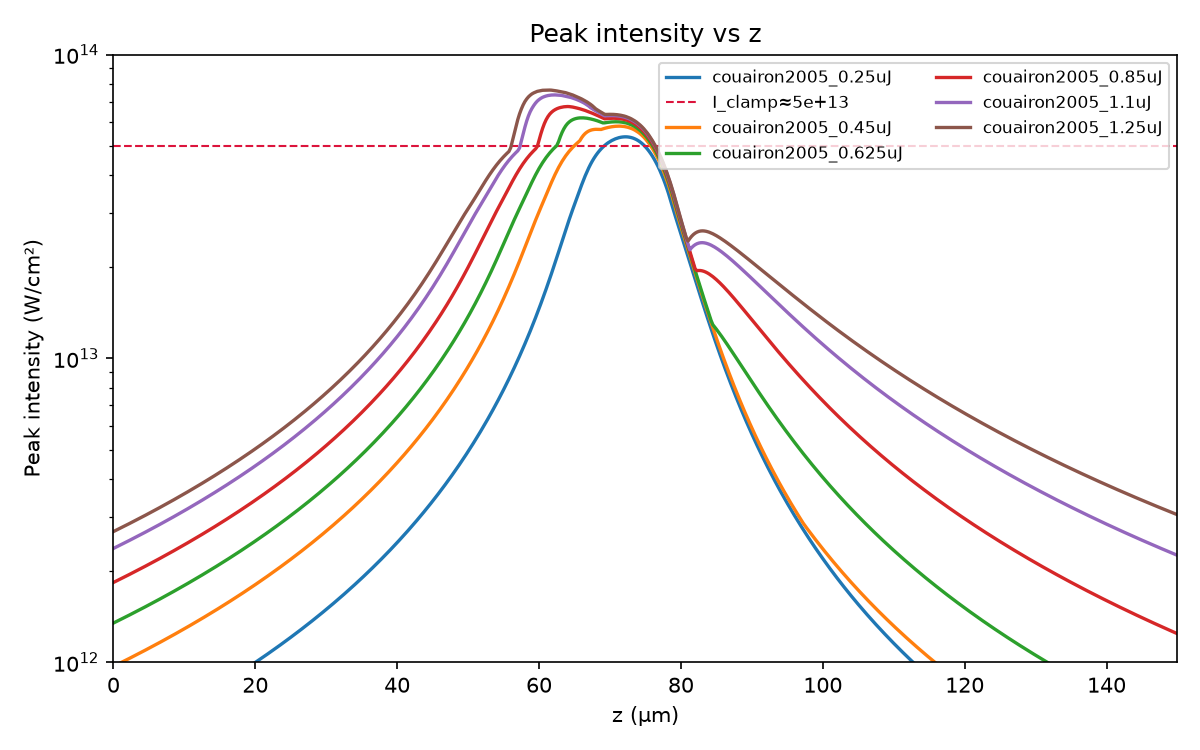
\includegraphics[width=0.85\linewidth]{couairon2005_fig8_energy_sweep.png}
    \caption{Peak on-axis intensity along $z$ for six input pulse energies from $0.25$ to $1.25\ \mu$J, reproducing Fig.~8 of~\cite{PhysRevB.71.125435}. Below threshold the peak intensity simply follows linear focusing (lower curves never reach $I_{clamp}$). Above it, every curve saturates at essentially the same value close to the clamping intensity $I_{clamp}\approx5\times10^{13}\ \text{W/cm}^2$ (dashed line) predicted from the intensity-clamping balance of Section~1.3.4 of the Couairon notes, before decaying on the trailing side of the nonlinear focus. This saturation, common to all above-threshold energies despite their different $P_{in}/P_{cr}$ ratios, is the numerical signature of intensity clamping referred to throughout Section~8.2.}
    \label{fig:fig8_peak_intensity}
\end{figure}

\FloatBarrier
\subsection{Cross-Validation Against Independent Simulations}

The figures above reproduce the specific published results of~\cite{PhysRevB.71.125435} at their exact laser parameters, as a check that the solver reproduces a result it was not tuned against. This subsection adds two further independent checks: a second published simulation with an entirely different parametrization, and an ablation of the propagation equation itself on the experiment actually used throughout this report.

\begin{figure}[htbp]
    \centering
    
\includegraphics[width=0.95\linewidth]{fig11.png}
    \caption{Fluence, absorbed energy density, peak intensity and electron density maps for the conditions of Bulgakova, Stoian \& Rosenfeld ($800\ \text{nm}$, $120\ \text{fs}$, $1\ \mu$J, $w_0=0.9\ \mu$m, geometric focus at $90\ \mu$m below the surface, dashed white line), a parametrization independent of~\cite{PhysRevB.71.125435} (different $n_2$, effective mass, collision time and lattice density). White contours mark the levels published in that reference; the solver's own fields (colour maps) fall within them across all four panels, including the secondary lobe past the geometric focus visible in panels (a)-(c), itself a signature of the refocusing cycle of Fig.~\ref{fig:filamentation_schematic}.}
    \label{fig:bulgakova_fig11}
\end{figure}

\begin{figure}[htbp]
    \centering
    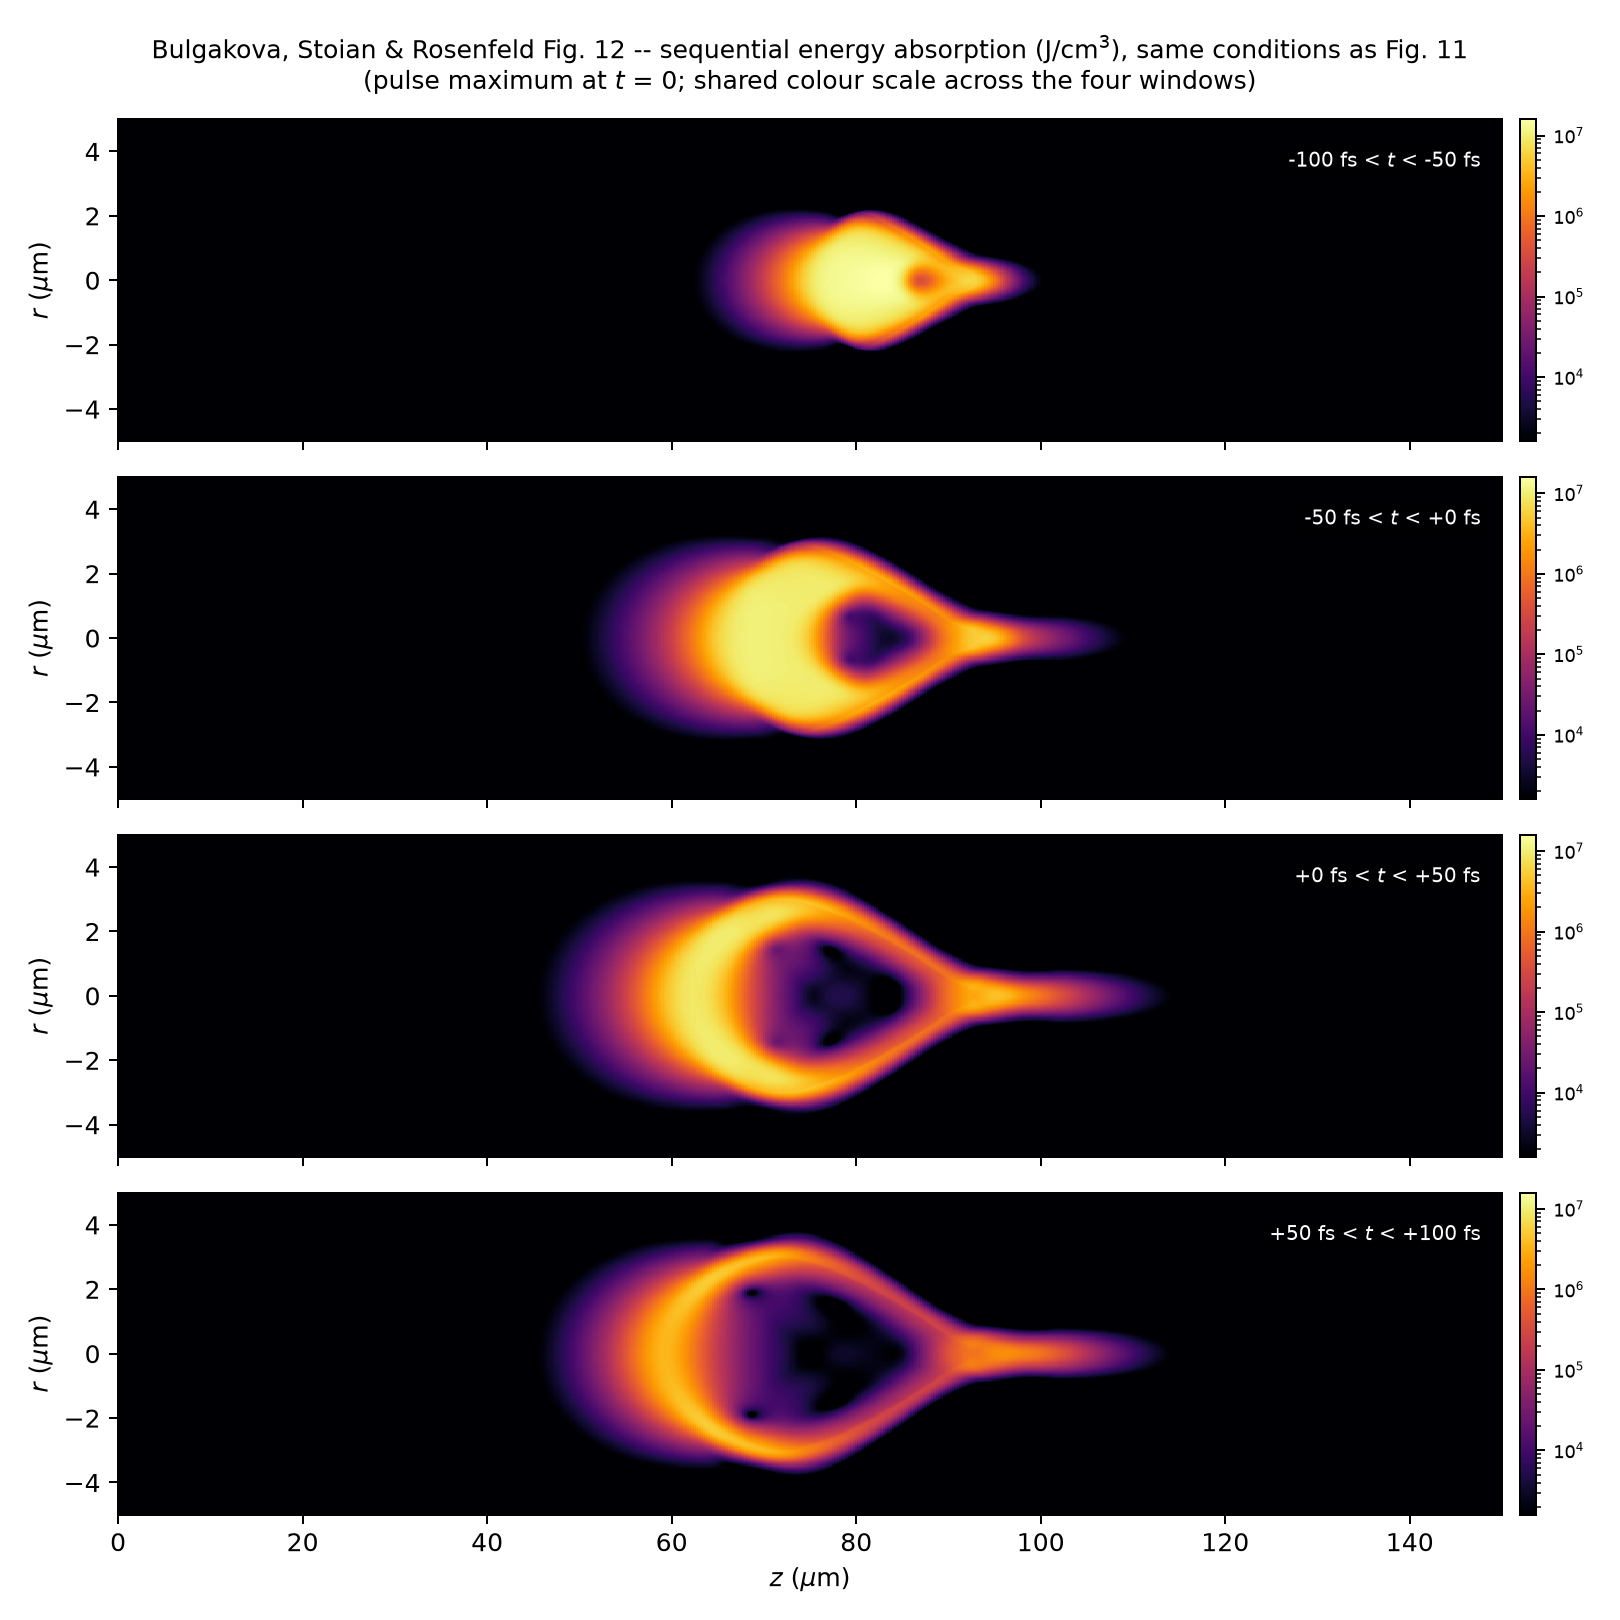
\includegraphics[width=0.95\linewidth]{fig12.png}
    \caption{Energy absorbed in four successive $50\ \text{fs}$ windows of the same pulse as Fig.~\ref{fig:bulgakova_fig11}, on a shared colour scale. Absorption is confined to a compact region near the pulse peak in the first window, then spreads into a hollow, ring-shaped pattern reaching further upstream (toward smaller $z$) in the later windows, consistent with plasma generated earlier in the pulse pre-absorbing and defocusing the beam before it reaches material deeper along the propagation axis.}
    \label{fig:bulgakova_fig12}
\end{figure}

\begin{figure}[htbp]
    \centering
    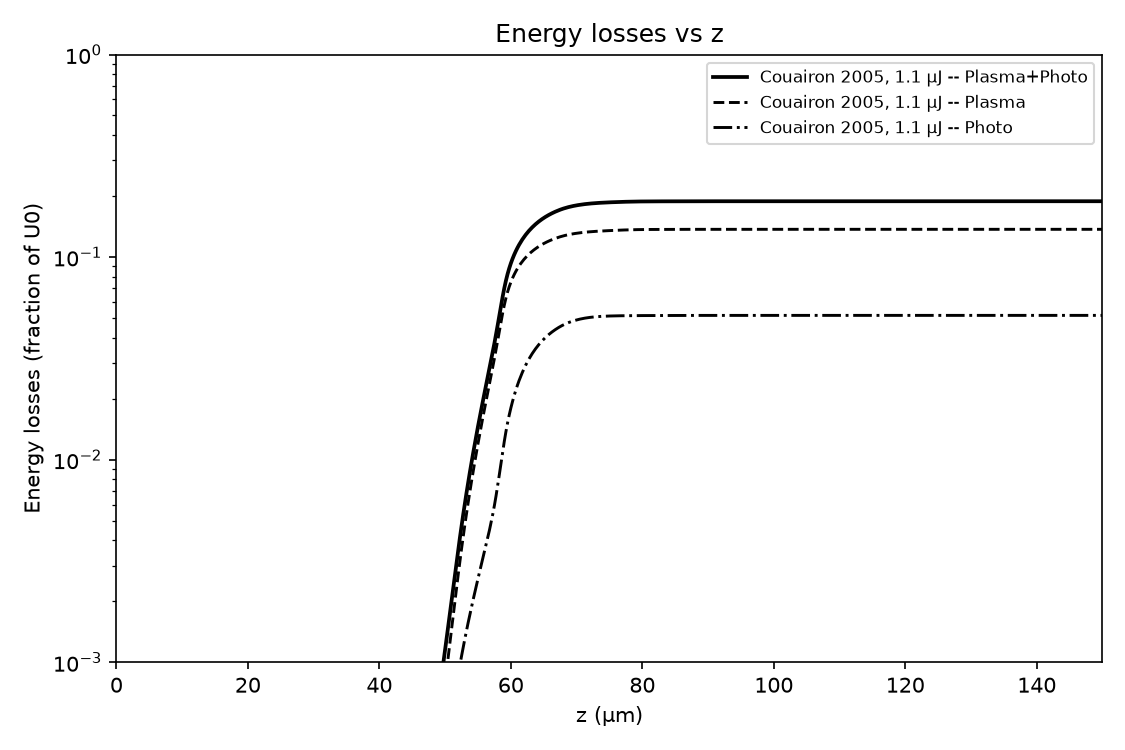
\includegraphics[width=0.8\linewidth]{fig12_energy_losses.png}
    \caption{Cumulative energy lost by the pulse of~\cite{PhysRevB.71.125435} (at $1.1\ \mu$J) as it propagates, as a fraction of the input energy $U_0$, separated into the plasma absorption and photoionization channels. Both losses turn on together at the nonlinear focus and saturate once the beam has defocused past the clamping intensity, plasma absorption (inverse bremsstrahlung on already-free carriers) accounting for roughly $2.5\times$ more of the total loss than direct photoionization, consistent with the two channels' relative weight, $\sigma_\omega/U_i$ against $W_{PI}/\rho_{at}$, discussed in Section~4.}
    \label{fig:energy_losses}
\end{figure}

\begin{figure}[htbp]
    \centering
    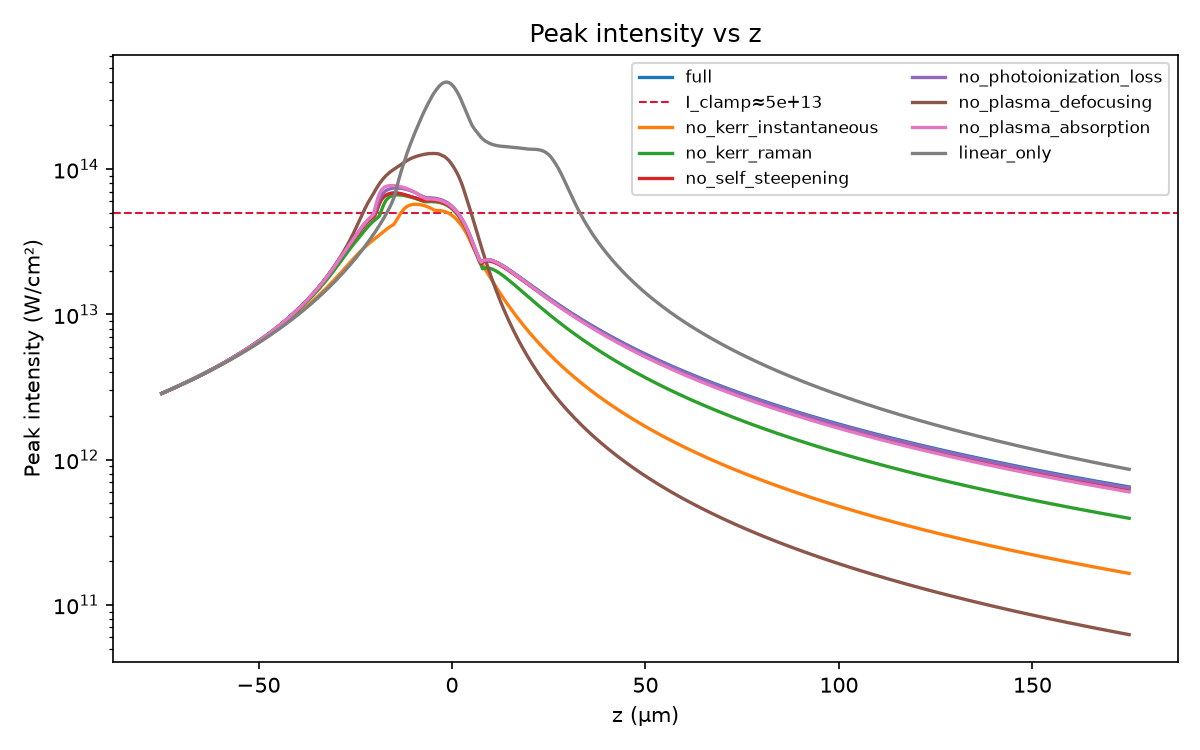
\includegraphics[width=0.85\linewidth]{comparison_fig8_peak_intensity.png}
    \caption{Peak on-axis intensity along $z$ for the experiment actually used throughout this report ($1030\ \text{nm}$, $263\ \text{fs}$, $15\ \mu$J, self-trapped exciton channel active), with each physical term of Eq.~\eqref{eq:master_propagation} disabled in turn. \texttt{linear\_only} (pure diffraction and dispersion, no Kerr, no plasma) overshoots the clamping intensity by nearly an order of magnitude, confirming that the balance discussed in Section~8.1 is what limits the intensity in every other curve. \texttt{no\_plasma\_defocusing} keeps the ionization losses but removes the defocusing phase, and reaches roughly twice the clamping intensity before the accumulated photoionization and avalanche losses alone eventually arrest it, showing that defocusing, not absorption, does most of the clamping work. \texttt{no\_kerr\_instantaneous} and \texttt{no\_kerr\_raman} both peak lower than \texttt{full} and decay markedly faster past the nonlinear focus, roughly an order of magnitude below \texttt{full} by $z=150\ \mu$m, consistent with the weaker Kerr response lengthening $L_c$ of Eq.~\eqref{eq:marburger}. The remaining curves (no self-steepening, no photoionization loss, no plasma absorption) are visually indistinguishable from \texttt{full} at this scale, since none of them changes the dominant balance between Kerr self-focusing and plasma defocusing that sets the clamping intensity itself.}
    \label{fig:comparison_fig8}
\end{figure}
\FloatBarrier
